\documentclass[a4paper]{article}
\usepackage[utf8]{inputenc}
\usepackage{a4wide}
\usepackage{url}
\usepackage{alltt}
\usepackage{graphicx}
\usepackage{libs/tex/abbrev_reactive}

\let\OldRightarrow=\Rightarrow
\RequirePackage{marvosym}
\let\MarvosymRightarrow=\Rightarrow
\let\Rightarrow=\OldRightarrow
\RequirePackage{wasysym}
\let\Lightning\UnTrucIndefini% Because conflict between ifsym and marvosym
\let\Sun\UnTrucIndefini%
\RequirePackage[weather]{ifsym}


\sloppy

\begin{document}

\title{Par4All Command Line Interface\\
  \texttt{p4a}\\
  ---\\
  HPC Project}

\author{Ronan \textsc{Keryell} \& Grégoire \textsc{Péan}}

\maketitle

\tableofcontents{}

% To automatically build reports from this content:
%%ContentBegin


\section{Introduction}
\label{sec:introduction}

\Apfa is a project aiming at easing code generation for various parallel
architectures from sequential source codes written in C or Fortran with
almost no manual code modification required. \Apfa is based on various
components such as the \Apips source-to-source compiler framework and is
mainly developed by \Ahpcp, Mines ParisTech and Institut Télécom. It
is open source to take advantage of a community effect and to avoid
capturing users in a proprietary short-term solution. Specialized target
developments and professional support are also available on demand.

The main interest of a source-to-source compiler is to be naturally
independent of the target very details and to take advantage of the best
back-end tools, such as highly optimized vendor compilers for a given
processor or platform, open-source compilers and tools, high-level
hardware synthesizers, \Acuda or \Aopencl compilers for \Agpu. At the same
time, some architectural aspects can be expressed or generated in some
special source constructs to capture architectural details when needed
(\Asimd or accelerators intrinsics). The source-to-source aspect makes
\Apfa \emph{de facto} interoperable with various other tools as front-end
or back-end to build complete tool chains.

\texttt{p4a} is the basic script interface to quickly use \Apfa for people
not interested in all the \Apips details but produce parallel code from
user sources.

This script can take C or Fortran source files and generate \Aopenmp or
\Acuda output to run respectively on shared memory multicore processors or
\Agpu.

The output is created into local \texttt{...p4a...} files extracted from a
temporary \texttt{\emph{x}.database} directory that can be optionally kept
for inspection as with any \Apips usage.

This script can also be used to call a back-end compiler such as
\texttt{gcc}, \texttt{icc} or \texttt{nvcc} to directly generate a binary
executable and you can choose many compiler and preprocessor options.

A CMake build infrastructure can be automatically generated to ease
further compilation by the back-end when running with the correct options.

The \Apfa documentation is available from \url{http://www.par4all.org} and
more specifically, this one can be found in \Apdf from
\url{http://download.par4all.org/doc/simple_tools/p4a/p4a_script.pdf}

Since \Apfa is a large project in continuous progress, you should refer to
release note and more generally on \url{http://www.par4all.org} to know
about the current status and limitations of the tools.

This project is funded through various research projects : French ANR
FREIA, European ARTEMIS SCALOPES, French Images and Network TransMedi@,
French System@tic OpenGPU, French ANR MediaGPU, European ARTEMIS SMECY.


\section{Examples and use cases of \protect\texttt{p4a}}
\label{sec:examples}

\subsection{Automatic parallelization with OpenMP generation}
\label{sec:autom-parall-with}

You want to generate some \Aopenmp code from a Fortran program:
\begin{verbatim}
p4a --openmp example.f
\end{verbatim}
and the output is in the \texttt{example.p4a.f}. Since it is the default
behavior, you can elide the \verb/--openmp/ option. The compilation
process transforms automatically data-parallel \emph{do}-loops into
\Aopenmp parallel loops with the correct pragmas and privatization of
scalar variables.


\subsection{Automatic parallelization with CUDA generation}
\label{sec:autom-parall-with-1}

To generate from a C program source a \Acuda program that is also compiled
into an executable:
\begin{verbatim}
p4a --cuda example.c -o e
\end{verbatim}
produces an \texttt{example.p4a.cu} \Acuda program source and an
\texttt{e} executable that will execute on a \Agpu. The \Agpu accelerator
support relies on a small \Apfa Accel interface that connects to the
\Acuda infrastructure. Data-parallel loops are automatically transformed
into \Acuda kernels that execute on the \Agpu with generation of \emph{ad
  hoc} communications between the host memory and the \Agpu memory.

To generate an \Aopenmp emulation executable of \Agpu-like accelerated
code (that ease with to ease debugging or if you do not have a \Agpu), try:
\begin{verbatim}
p4a --accel --openmp example.c -o e
\end{verbatim}
there should be an \texttt{e} binary executable file with its
corresponding \texttt{example.p4a.c} program source. This \Aopenmp
emulation of \Acuda with memory transfer may be helpful to debug some code
since there is no longer emulation mode in recent version of \Acuda.

The interest of the source-to-source approach is that you can further
improve the generated code manually or use it as starting point for other
developments. When compiling the \Apfa Accel generated code, you can
define different preprocessor symbols according to the expected target:
\begin{itemize}
\item \verb|P4A_ACCEL_CUDA| preprocessor symbol, the source is to be
  compiled as \Acuda;
\item \verb|P4A_ACCEL_OPENMP| preprocessor symbol, the source is to be
  compiled as \Aopenmp or sequential emulation code.
\end{itemize}

You can avoid parallelizing some functions by using
\texttt{-{}-exclude-modules=\emph{regex}} when the parallel part is not
enough compute-intensive since transferring data and launching a kernel
may be more expensive than sequential execution.

There is also an option to exclude some files from the back-end
compilation, for example if you want to use already optimized library. For
this you analyze your program by providing stubs definitions in a file
that are dummy function definitions that have a similar global memory
effect so that \Apips global interprocedural analysis are happy and just
in the back-end stage you skip this file with \verb|--exclude-file|, then
replace the dummy calls by the real library functions, by linking with
them with \texttt{-l} or compiling them with \verb|--extra-file|.


\subsubsection{P4A Accel runtime tweaking}
\label{sec:p4a-accel-runtime}

To ease code generation and portability, \Apfa does not directly generate
direct \Acuda code for example. It generates calls to functions and
macrofunctions defined in the P4A Accel runtime.

There are many parameters that can be changed to better suit a given
application on a given target.

In the case of \Acuda generation, you can pass flags to the \texttt{nvcc}
back-end compiler with the \verb|--nvcc-flags=...| option.

For example
\begin{itemize}
\item if you want to debug the output with \texttt{cuda-gdb}, use
  \verb|--nvcc-flags="-g -G"|;
\item to optimize the \Acuda code with \verb|--nvcc-flags=-O3|;
\item \verb|--nvcc-flags="-gencode arch=compute_20,code=sm_20"| to
  generate code to Fermi board;
\item
  \verb|--nvcc-flags="-gencode arch=compute_10,code=sm_10 -gencode arch=compute_20,code=sm_20"|
  to generate code to both Tesla \& Fermi board.
\end{itemize}

You can debug the P4A Accel runtime itself with
\verb|--nvcc-flags=-DP4A_DEBUG| to output debugging messages around all
the \Acuda kernels invocations, such as: {\scriptsize
\begin{verbatim}
 P4A: Calling 2D kernel "p4a_kernel_wrapper_0" of size (8192x8192)
 P4A: Creating grid of block descriptor "P4A_grid_descriptor" of size 16x8192x1
 P4A: Creating thread block descriptor "P4A_block_descriptor" of size 512x1x1
 P4A: line 43 of function p4a_kernel_launcher_0 in file ".../parameterized_kernel.p4a.cu":
 P4A: Invoking kernel (p4a_kernel_wrapper_0, P4A_grid_descriptor, P4A_block_descriptor) with (i, j, array)
\end{verbatim}
}

If you get at runtime some error message such as:
\begin{verbatim}
CUTIL CUDA error : P4A CUDA kernel execution failed :
too many resources requested for launch
\end{verbatim}
there is not enough registers to run all the requested threads in a block,
so you can try by relaunching \texttt{p4a} with a
\verb|--nvcc=-DP4A_CUDA_THREAD_MAX=384| or even less, instead the default
value of 512 threads per block.

You can select the maximum number of threads in a block of thread for 1D
kernels with a \verb|--nvcc-flags='-DP4A_CUDA_THREAD_PER_BLOCK_IN_1D=...|

For 2D kernels, you can set the \verb|P4A_CUDA_THREAD_X_PER_BLOCK_IN_2D|
and \verb|P4A_CUDA_THREAD_Y_PER_BLOCK_IN_2D| in the same way. For
efficiency reasons, on nVidia \Agpu, the threads are first allocated along
the $X$ dimension (the \emph{warp} dimension) and once the
\verb|P4A_CUDA_THREAD_X_PER_BLOCK_IN_2D| limit is reached, it is allocated
along the $Y$ dimension. Right now, parallel loop nests that are
parallelized have their parallelism then limited up to 2 dimensions to
cope more easily with \Acuda \Agpu hardware limitation. The outer-loop is
mapped on the $X$ \Agpu dimension, so it is the dimension that must have
enough parallelism.

For more tweaking, look at the \Apfa Accel runtime source on \url{} or
directly in the \Agit repository.


\section{p4a full option list}
\label{sec:options}

The basic usage is \texttt{p4a [\emph{options}] <\emph{source files}>}

The following documentation is automatically generated from the
\texttt{p4a} source code.

\input{p4a-help}

\section{p4a architecture}
\label{sec:p4a-architecture}

The global architecture of \Apfa is given on
figure~\ref{fig:transit_intestinal}.

\begin{figure}
  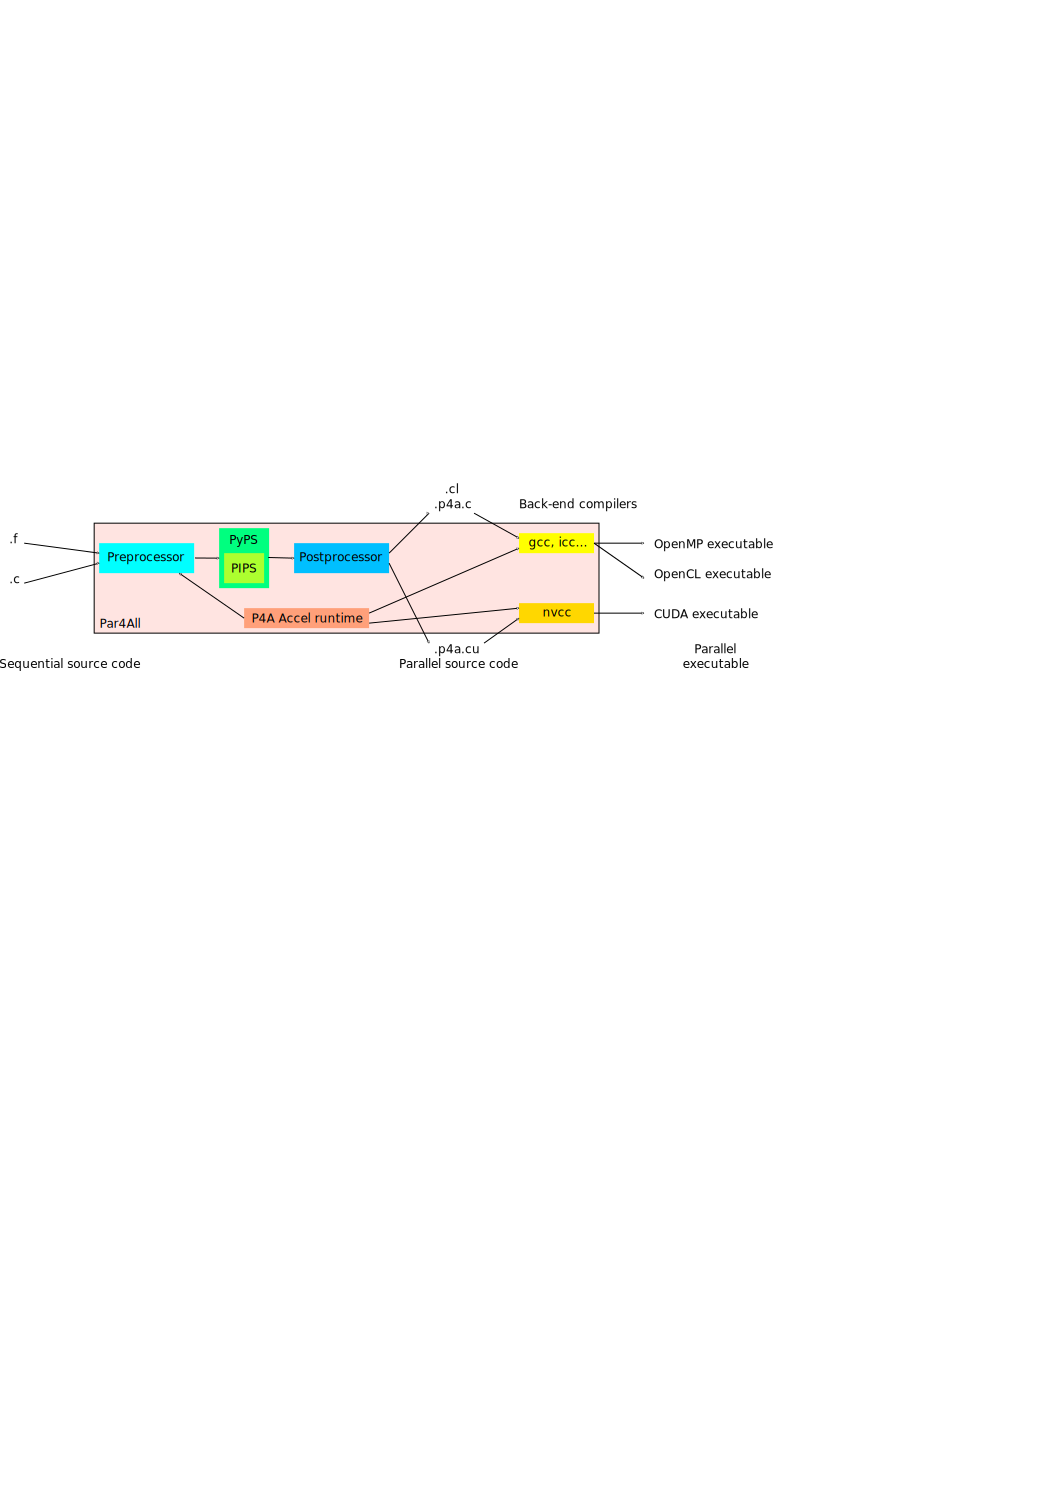
\includegraphics[width=\hsize]{p4a_work_flow}
  \caption{Intestinal view of \texttt{p4a}.}
  \label{fig:transit_intestinal}
\end{figure}

%%ContentEnd

\end{document}


%%% Local Variables:
%%% mode: latex
%%% ispell-local-dictionary: "american"
%%% End:

